\documentclass[UTF8,a4paper,12pt,fontset=none]{ctexart}

\usepackage[a4paper,margin=2.2cm]{geometry}
\usepackage{array}
\usepackage{booktabs}
\usepackage{caption}
\usepackage{enumitem}
\usepackage{float}
\usepackage{fontspec}
\usepackage{graphicx}
\usepackage{hyperref}
\usepackage{listings}
\usepackage{siunitx}
\usepackage{subcaption}
\usepackage{tabularx}
\usepackage{xcolor}

\hypersetup{colorlinks=true,linkcolor=blue!60!black,urlcolor=blue!60!black}
\defaultCJKfontfeatures{AutoFakeSlant=.2}
\setmainfont[SlantedFont=Times New Roman Italic,BoldItalicFont=Times New Roman Bold Italic]{Times New Roman}
\setCJKmainfont[SlantedFont=Songti SC]{Songti SC}
\setCJKsansfont{Heiti SC}
\setCJKmonofont{Heiti SC}
\setmonofont{Menlo}
\setlength{\parindent}{2em}
\setlength{\parskip}{0.35em}
\graphicspath{{../results/figures/}{results/figures/}}
\captionsetup{font=small}
\sisetup{round-mode=places,round-precision=3}
\renewcommand{\figurename}{图}
\renewcommand{\tablename}{表}

\definecolor{AccentA}{HTML}{0B6E4F}
\definecolor{AccentB}{HTML}{1D4E89}
\definecolor{AccentC}{HTML}{F4A259}
\definecolor{AccentD}{HTML}{C73E1D}
\definecolor{CodeBg}{HTML}{F7F7F7}

\title{\bfseries 中山大学计算机学院本实验报告}
\author{}
\date{}

\begin{document}

\begin{titlepage}
  \centering
  {\zihao{2}\bfseries 中山大学计算机学院本实验报告\par}
  \vspace{0.5em}
  {\zihao{4}（2025学年春季学期）\par}
  \vspace{2em}

  \begin{tabularx}{0.9\textwidth}{>{\bfseries}p{4cm}X}
    课程名称： & 并行程序设计与算法 \\
    实验题目： & Lab3 基于 Pthreads 的并行矩阵乘法与数组求和 \\
    学号： & 23336128 \\
    姓名： & 梁力航 \\
    完成日期： & 2026年4月16日 \\
  \end{tabularx}

  \vfill
  \begin{minipage}{0.88\textwidth}
    \small
    本报告围绕 Lab3 的两项任务展开：一是使用 Pthreads 实现并行矩阵乘法，并比较“连续行块静态划分”和“循环行分配”两种划分方式；二是实现并行数组求和，并比较“每线程局部和 + 主线程归并”与“mutex 保护共享总和”两种归约方式。实验目标不是单纯证明线程数越多越快，而是分析线程划分、归约竞争以及内存访问模式如何共同影响性能与可扩展性。
  \end{minipage}
\end{titlepage}

\section{实验目的}

本实验的目标包括：
\begin{enumerate}[leftmargin=2.2em]
  \item 实现两个版本的 Pthreads 矩阵乘法：\texttt{v1\_row\_block} 与 \texttt{v2\_cyclic\_rows}；
  \item 实现两个版本的 Pthreads 数组求和：\texttt{v1\_local\_sum} 与 \texttt{v2\_mutex\_shared\_sum}；
  \item 在不同线程数和不同问题规模下完成 benchmark，生成运行时间、加速比和并行效率结果；
  \item 形成自动化 benchmark、图表、表格与中文报告的闭环，保证结果可复现、可解释、可提交。
\end{enumerate}

\section{实验平台与环境}

本实验在 Apple Silicon 本机环境完成，统一使用 \texttt{uv} 管理 Python 脚本依赖。实验环境如下。

\begin{table}[H]
  \centering
  \caption{实验环境信息}
  \renewcommand{\arraystretch}{1.2}
  \begin{tabularx}{0.92\textwidth}{>{\bfseries}p{4cm}X}
    \toprule
    项目 & 配置 \\
    \midrule
    操作系统 & macOS / Darwin 25.3.0 \\
    CPU 架构 & Apple Silicon (arm64) \\
    C++ 编译器 & clang++，C++17，\texttt{-pthread} \\
    Python 工作流 & \texttt{uv run python ...} \\
    默认随机种子 & \texttt{20250401} \\
    结果输出契约 & 稳定 \texttt{key=value} \\
    \bottomrule
  \end{tabularx}
\end{table}

这里需要说明两点。第一，矩阵乘法与数组求和都沿用固定 seed，以保证不同线程数和不同版本之间的结果可比。第二，程序支持 \texttt{--dump}，但仅用于小规模调试；正式 benchmark 只保留结构化字段，避免结果文件被原始数据污染。

\section{实验过程与核心实现}

\subsection{矩阵乘法：两种线程划分方式}

矩阵乘法的目标是计算 \(C=A\times B\)。本实验实现了两个版本。

\begin{enumerate}[leftmargin=2.2em]
  \item \textbf{v1\_row\_block}：将矩阵 \(A\) 的行按连续区间分配给不同线程，每个线程独立计算自己负责的行块；
  \item \textbf{v2\_cyclic\_rows}：将行索引按 \texttt{row \% threads} 进行循环分配，以提高负载均衡，但会打散访存局部性。
\end{enumerate}

连续行块划分的优势在于线程访问的 \(A\) 和 \(C\) 区域更集中，更容易保持缓存友好；循环行分配在理论上更均衡，但它会让线程访问模式变得更离散，在大规模矩阵下更容易暴露缓存和带宽压力。

\subsection{数组求和：两种归约方式}

数组求和的目标是计算 \(S=\sum_i a_i\)。本实验实现了两种版本。

\begin{enumerate}[leftmargin=2.2em]
  \item \textbf{v1\_local\_sum}：每个线程先计算自己的局部和，全部线程结束后由主线程顺序合并；
  \item \textbf{v2\_mutex\_shared\_sum}：每个线程计算出局部和后，通过 \texttt{mutex} 将结果累加到共享变量。
\end{enumerate}

这两个版本的主要区别不是“算术计算”本身，而是归约时是否引入锁竞争。v1 把竞争降到最低；v2 则更直接，但在高线程数下更容易受同步开销影响。

\section{Benchmark 设计与正确性校验}

\subsection{测试范围}

本实验使用如下 benchmark 维度：
\begin{itemize}
  \item 矩阵乘法规模：\(128,256,512,1024,2048\)
  \item 数组求和长度：\(1\text{M},2\text{M},4\text{M},8\text{M},16\text{M},32\text{M},64\text{M},128\text{M}\)
  \item 线程数：\(1,2,4,8,16\)
  \item 每组重复次数：3
  \item 固定随机种子：20250401
\end{itemize}

\subsection{正确性校验}

benchmark 脚本会对每组配置进行如下检查：
\begin{enumerate}[leftmargin=2.2em]
  \item 程序返回码必须为 0；
  \item stdout 必须包含完整的 \texttt{key=value} 字段；
  \item 同一配置多次运行时，矩阵乘法的 \texttt{checksum/max\_abs} 必须一致；
  \item 同一配置多次运行时，数组求和的 \texttt{sum} 必须一致；
  \item 再基于单线程结果计算 speedup 与 efficiency，用于后续分析。
\end{enumerate}

\section{关键结果摘要}

为了避免只看曲线、不看定量结果，表\ref{tab:key-results} 汇总了最有代表性的四组配置。可以看到，本实验的结论并不是“线程数越多越好”，而是不同任务在不同规模下，会对划分方式与同步策略表现出明显不同的敏感性。

\begin{table}[H]
  \centering
  \small
  \caption{代表性配置结果摘要}
  \label{tab:key-results}
  \renewcommand{\arraystretch}{1.18}
  \begin{tabularx}{0.96\textwidth}{>{\raggedright\arraybackslash}p{3.1cm} >{\centering\arraybackslash}p{2.8cm} >{\centering\arraybackslash}p{1.2cm} >{\centering\arraybackslash}p{1.7cm} >{\centering\arraybackslash}p{1.7cm} >{\raggedright\arraybackslash}X}
    \toprule
    版本 & 规模 & 线程数 & $T_1$ (s) & $T_{16}$ (s) & 16线程加速比 / 效率 \\
    \midrule
    v1 row block & $2048\times2048\times2048$ & 16 & 27.560 & 9.176 & 3.003 / 0.188 \\
    v2 cyclic rows & $2048\times2048\times2048$ & 16 & 23.452 & 10.077 & 2.327 / 0.145 \\
    v1 local sum & $128\text{M}$ & 16 & 0.0809 & 0.0139 & 5.825 / 0.364 \\
    v2 mutex shared sum & $128\text{M}$ & 16 & 0.0898 & 0.0182 & 4.947 / 0.309 \\
    \bottomrule
  \end{tabularx}
\end{table}

从表中可以直接读出两个重要结论。第一，在最大矩阵规模 \(2048\) 下，\texttt{v1\_row\_block} 的 16 线程运行时间比 \texttt{v2\_cyclic\_rows} 少 0.901 秒，领先约 \SI{8.9}{\percent}；对应加速比也更高（3.003 对 2.327），说明连续行块划分在大规模访存场景下更能保持稳定的局部性。第二，在 \(128\text{M}\) 数组求和上，\texttt{v1\_local\_sum} 比 \texttt{v2\_mutex\_shared\_sum} 快约 \SI{23.5}{\percent}，表明即使临界区只在局部和汇总时出现，mutex 同步开销仍然会削弱最终可扩展性。

不过，这种优势并非对所有规模都完全一致。以 \(512\) 规模为例，\texttt{v2\_cyclic\_rows} 的 16 线程时间为 0.0330 秒，略快于 \texttt{v1\_row\_block} 的 0.0340 秒。说明在中等规模下，循环分配带来的负载均衡，仍然可能弥补部分局部性损失。因此，本实验更准确的结论应当是：不同并行策略的优劣具有明显的规模依赖性，而不是存在一个对所有输入都绝对最优的版本。

\section{实验结果与可视化分析}

\subsection{矩阵乘法}

\begin{figure}[H]
  \centering
  \begin{subfigure}[t]{0.48\textwidth}
    \centering
    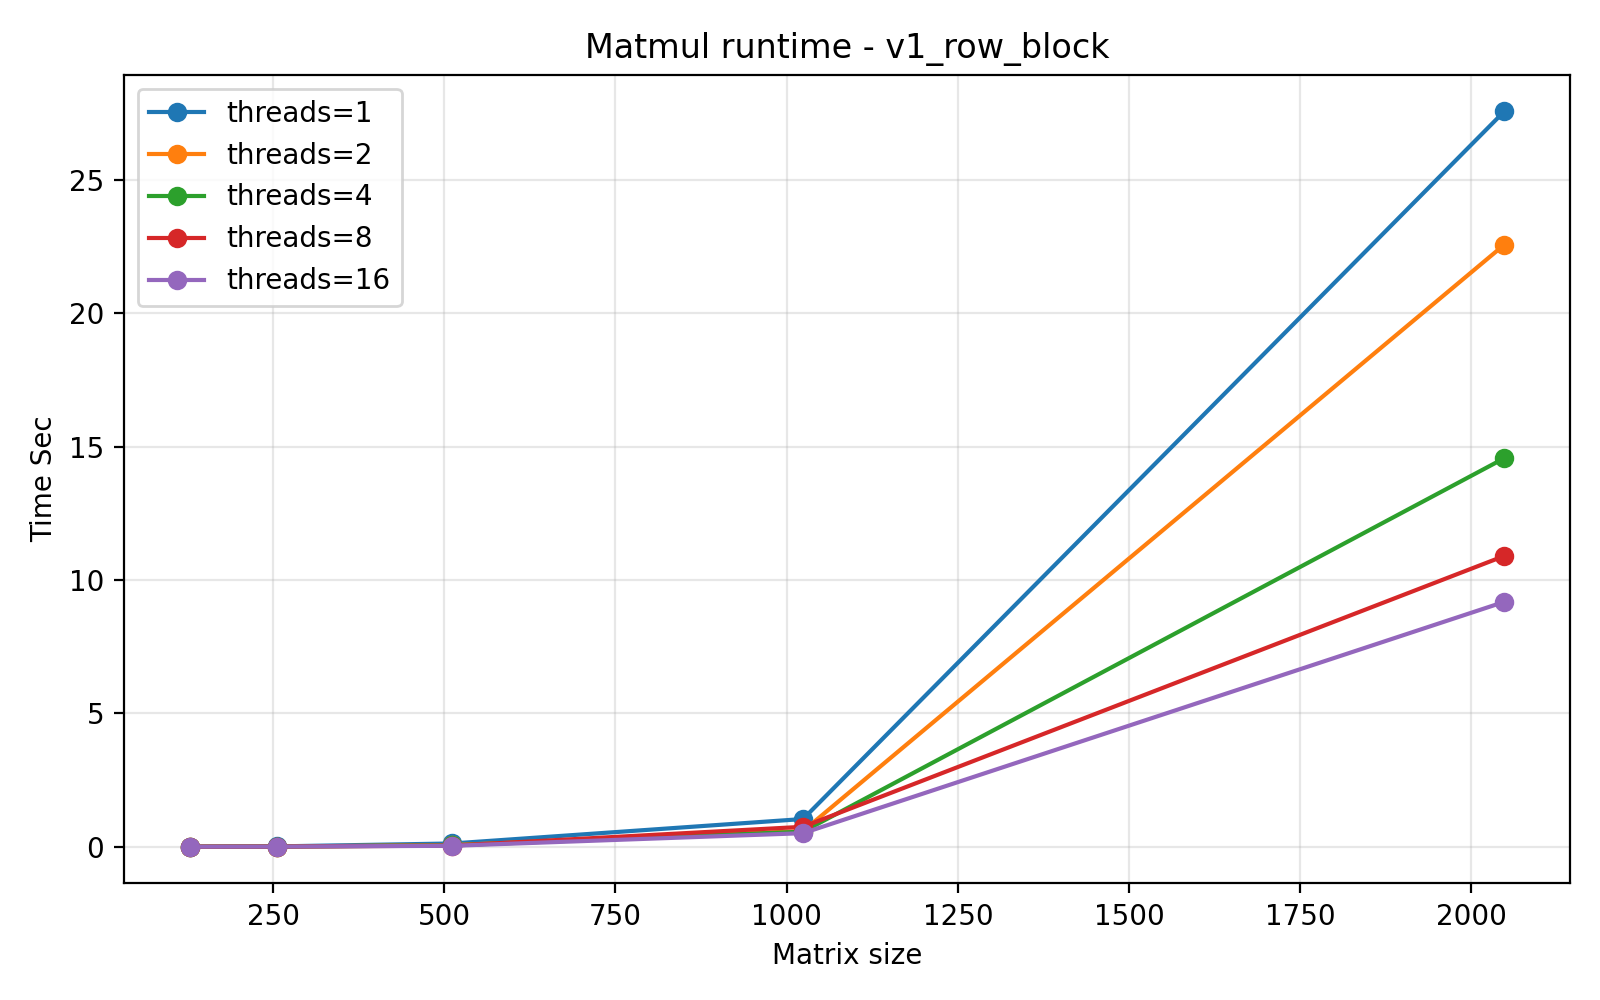
\includegraphics[width=\textwidth]{runtime_matmul_v1_row_block.png}
    \caption{\texttt{v1\_row\_block} 运行时间}
  \end{subfigure}
  \hfill
  \begin{subfigure}[t]{0.48\textwidth}
    \centering
    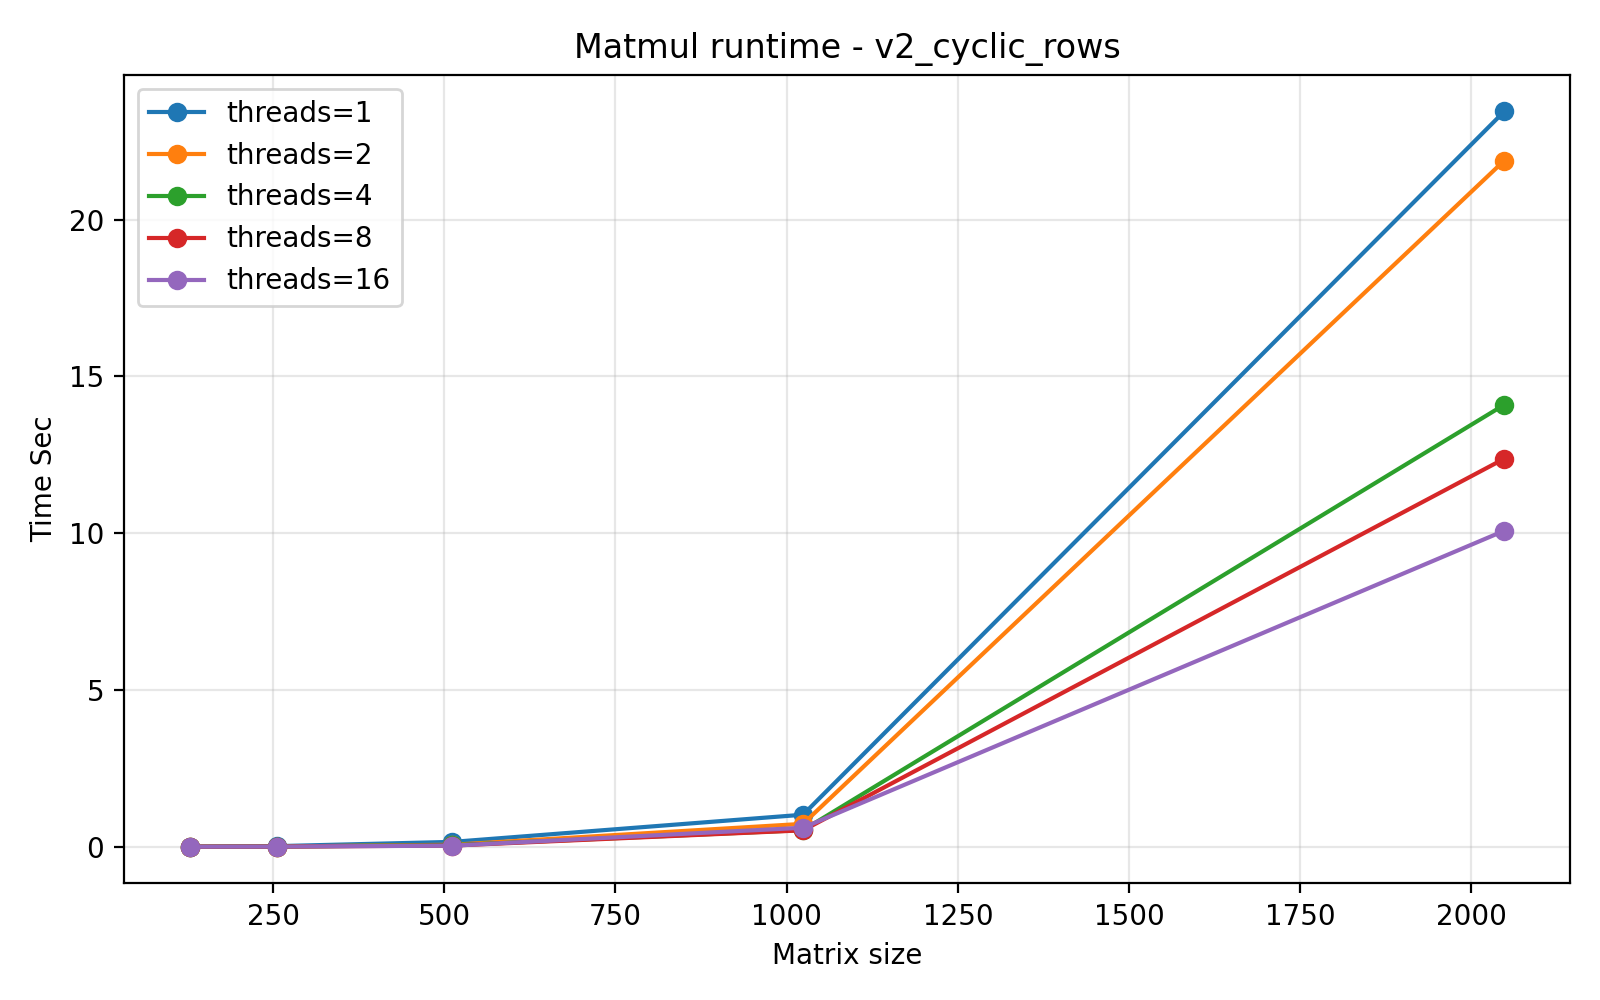
\includegraphics[width=\textwidth]{runtime_matmul_v2_cyclic_rows.png}
    \caption{\texttt{v2\_cyclic\_rows} 运行时间}
  \end{subfigure}
  \caption{矩阵乘法运行时间曲线}
\end{figure}

\begin{figure}[H]
  \centering
  \begin{subfigure}[t]{0.48\textwidth}
    \centering
    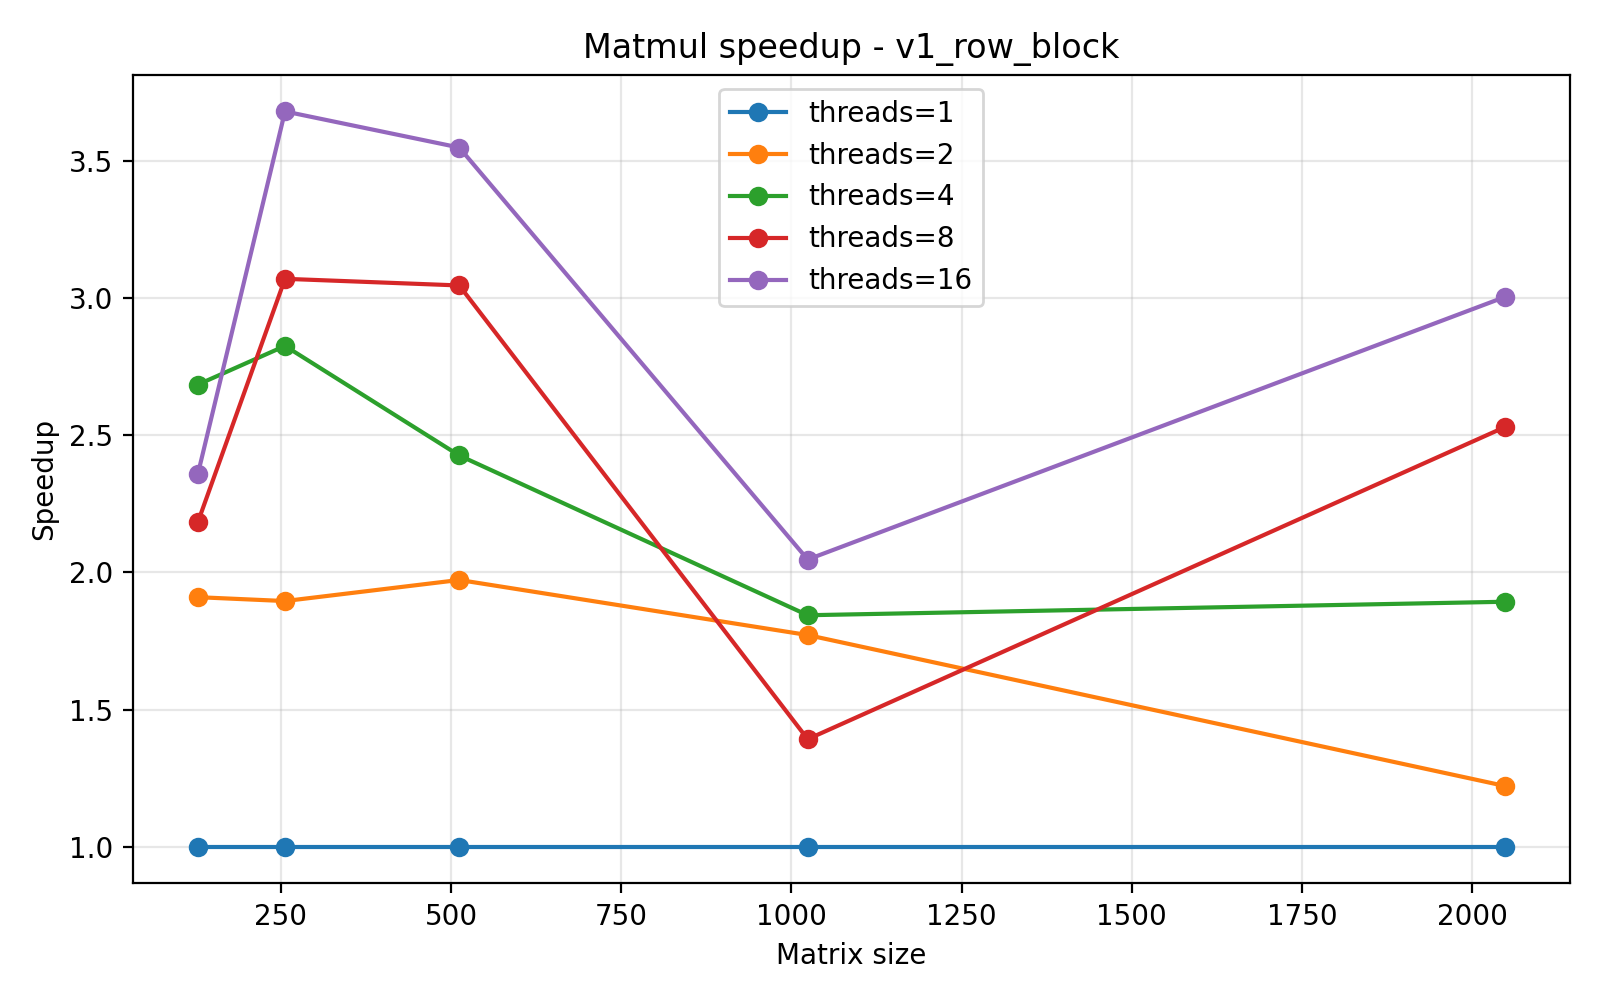
\includegraphics[width=\textwidth]{speedup_matmul_v1_row_block.png}
    \caption{\texttt{v1\_row\_block} 加速比}
  \end{subfigure}
  \hfill
  \begin{subfigure}[t]{0.48\textwidth}
    \centering
    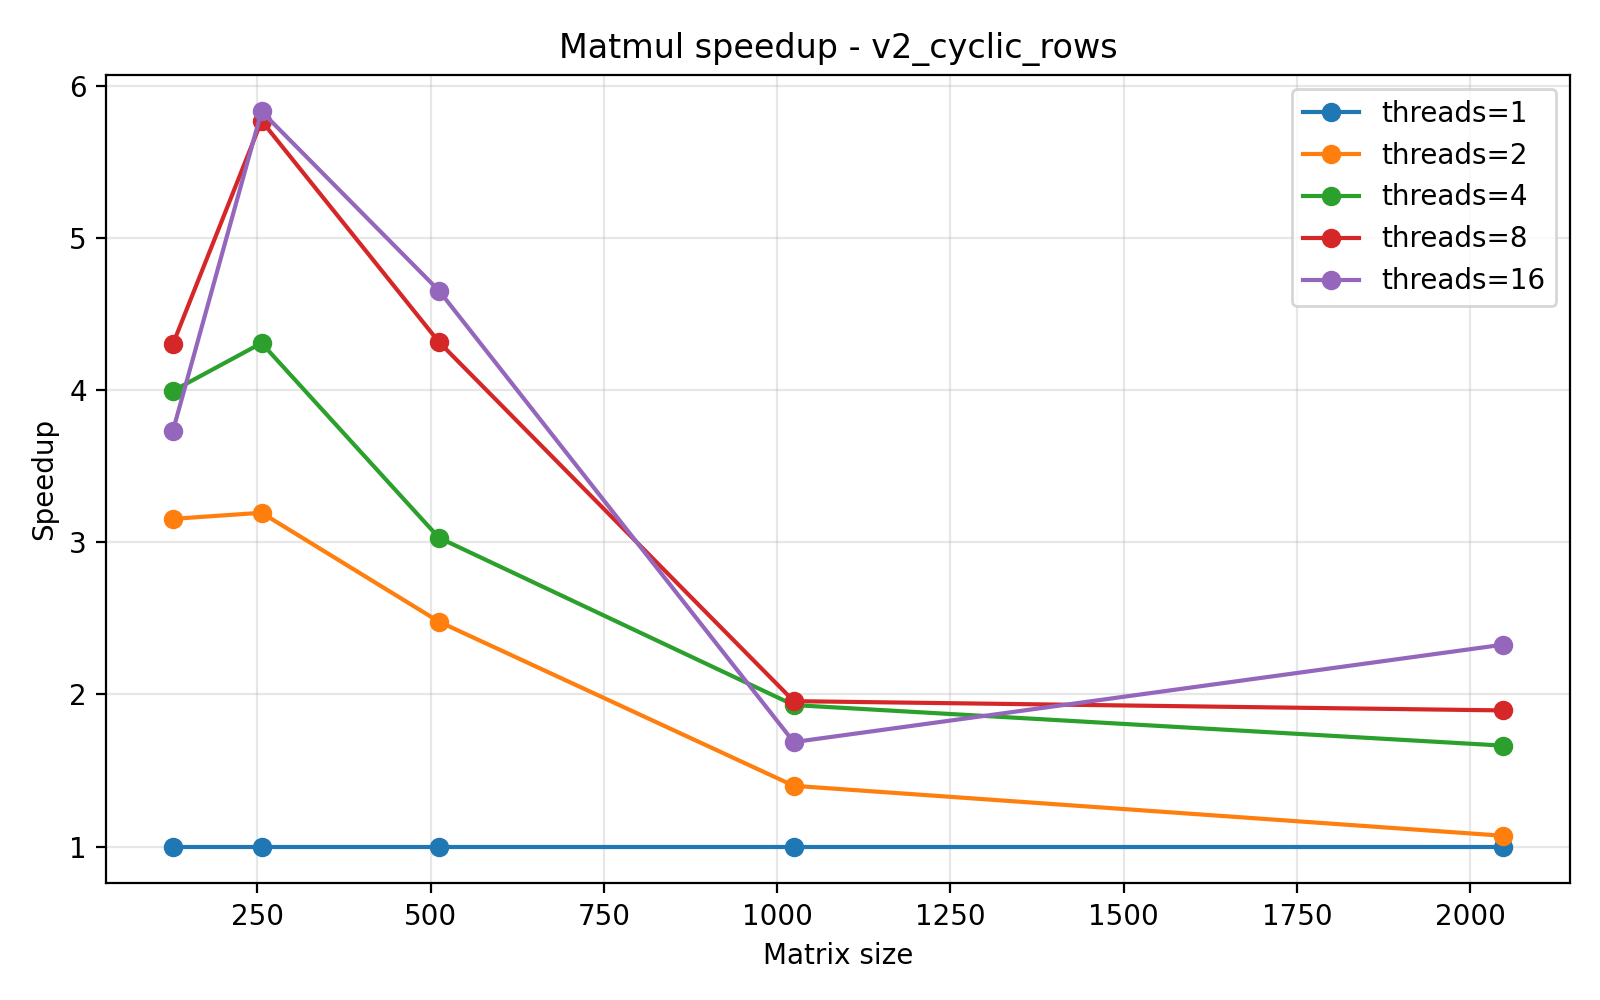
\includegraphics[width=\textwidth]{speedup_matmul_v2_cyclic_rows.png}
    \caption{\texttt{v2\_cyclic\_rows} 加速比}
  \end{subfigure}
  \caption{矩阵乘法加速比曲线}
\end{figure}

\begin{figure}[H]
  \centering
  \begin{subfigure}[t]{0.48\textwidth}
    \centering
    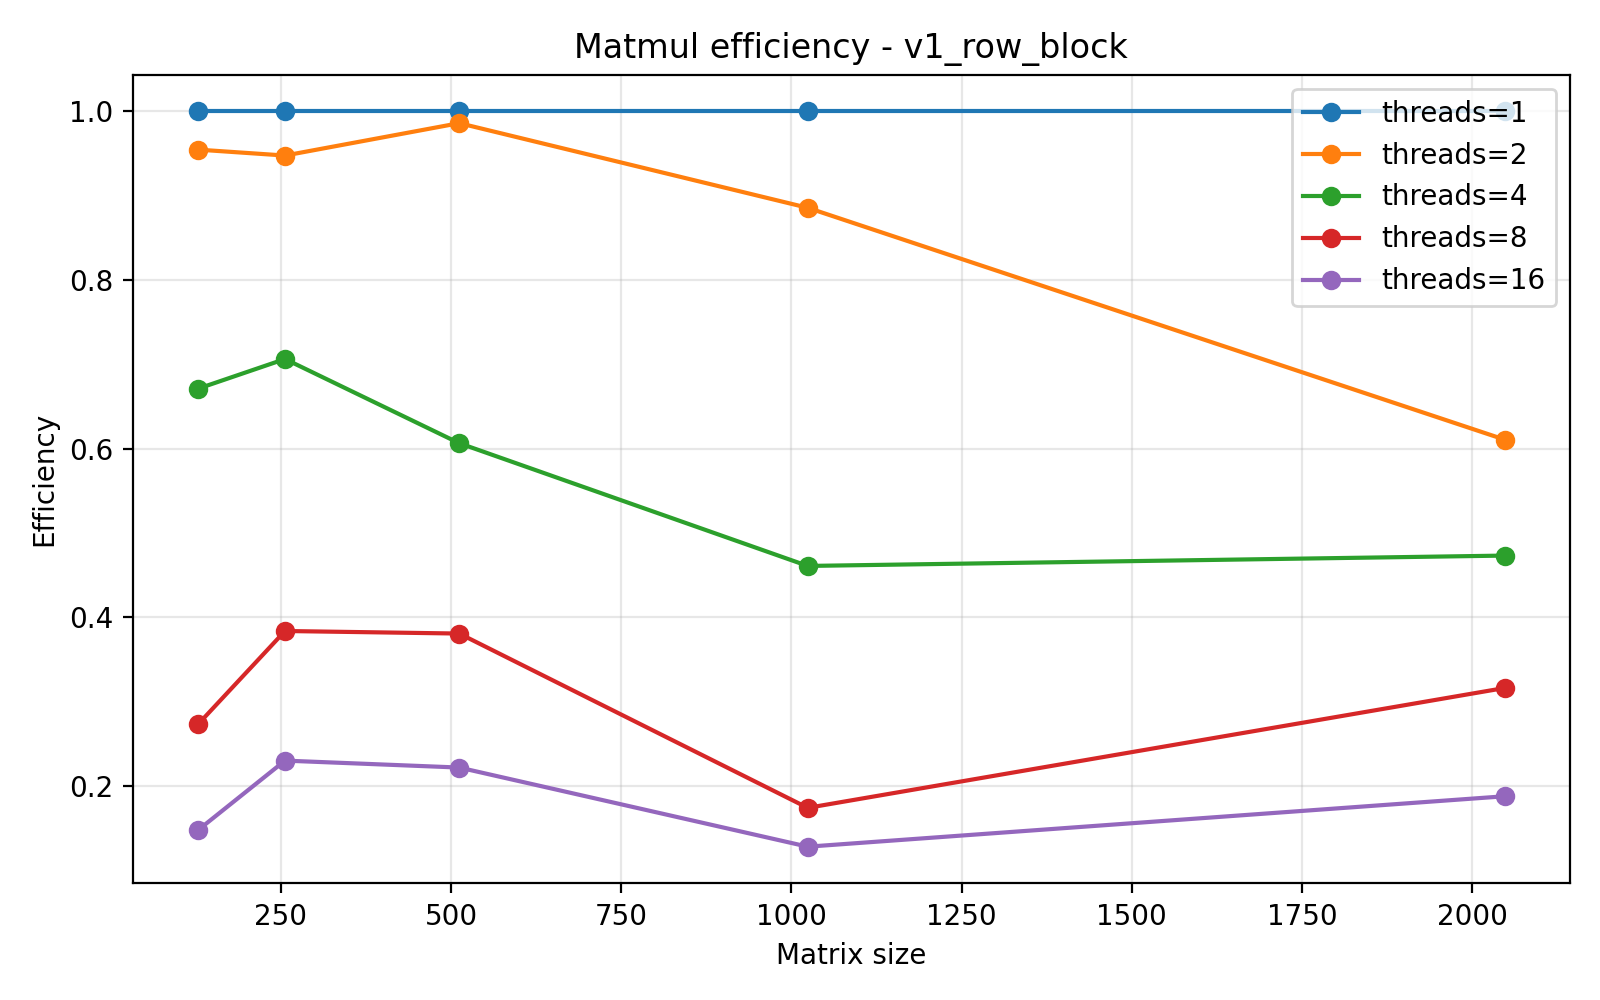
\includegraphics[width=\textwidth]{efficiency_matmul_v1_row_block.png}
    \caption{\texttt{v1\_row\_block} 并行效率}
  \end{subfigure}
  \hfill
  \begin{subfigure}[t]{0.48\textwidth}
    \centering
    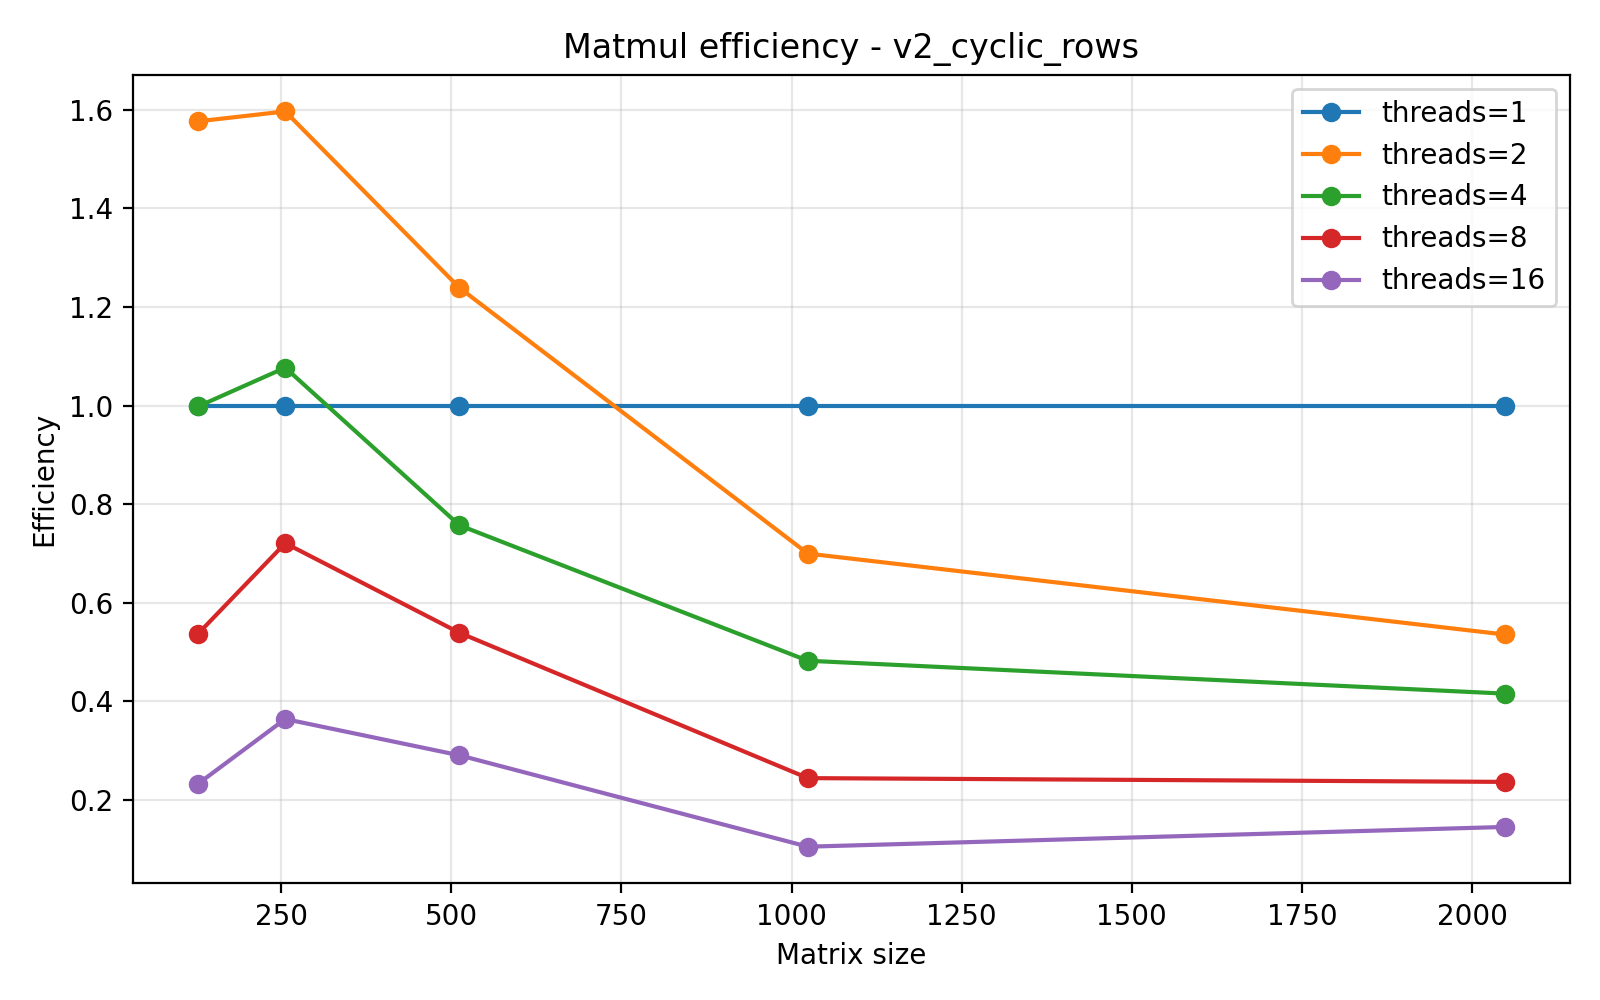
\includegraphics[width=\textwidth]{efficiency_matmul_v2_cyclic_rows.png}
    \caption{\texttt{v2\_cyclic\_rows} 并行效率}
  \end{subfigure}
  \caption{矩阵乘法并行效率曲线}
\end{figure}

矩阵乘法的结果表明，两种版本都能从多线程中获益，但收益并不是随线程数单调线性增长。若只看最大规模 \(2048\)，\texttt{v1\_row\_block} 从 1 线程到 16 线程的运行时间由 27.560 秒下降到 9.176 秒，speedup 为 3.003；\texttt{v2\_cyclic\_rows} 则由 23.452 秒下降到 10.077 秒，speedup 为 2.327。也就是说，虽然 \texttt{v2} 的单线程基线更快，但在高线程数下反而被 \texttt{v1} 反超，说明决定最终性能的并不只是计算均衡，还包括线程访问模式与缓存行为。

进一步看不同规模点，\texttt{v2\_cyclic\_rows} 并非始终落后。例如在 \(256\) 规模下，其 8 线程 speedup 达到 5.768，略高于 \texttt{v1\_row\_block} 的 3.070；在 \(512\) 规模下，\texttt{v2} 的 16 线程时间也略优于 \texttt{v1}。这说明当问题规模还没有大到完全受内存层次结构支配时，循环分配确实可能因为行工作量更均衡而获得阶段性优势。但随着规模扩大到 \(1024\) 和 \(2048\)，这种优势迅速减弱：在 \(2048\) 上，\texttt{v1} 的 16 线程效率为 0.188，而 \texttt{v2} 只有 0.145。这个差距说明，打散行访问会让线程对矩阵 \(A\) 与结果矩阵 \(C\) 的写入更加离散，从而削弱缓存命中率，最终抵消掉原本的负载均衡收益。

因此，矩阵乘法部分最重要的结论不是“循环分配不好”，而是：在这种以规则稠密计算为主、且单行计算量已经相对接近的场景里，连续行块静态划分往往能以更好的局部性换来更稳定的整体性能；而循环分配只有在中等规模、负载均衡收益尚能覆盖访存代价时才会局部占优。

\subsection{数组求和}

\begin{figure}[H]
  \centering
  \begin{subfigure}[t]{0.48\textwidth}
    \centering
    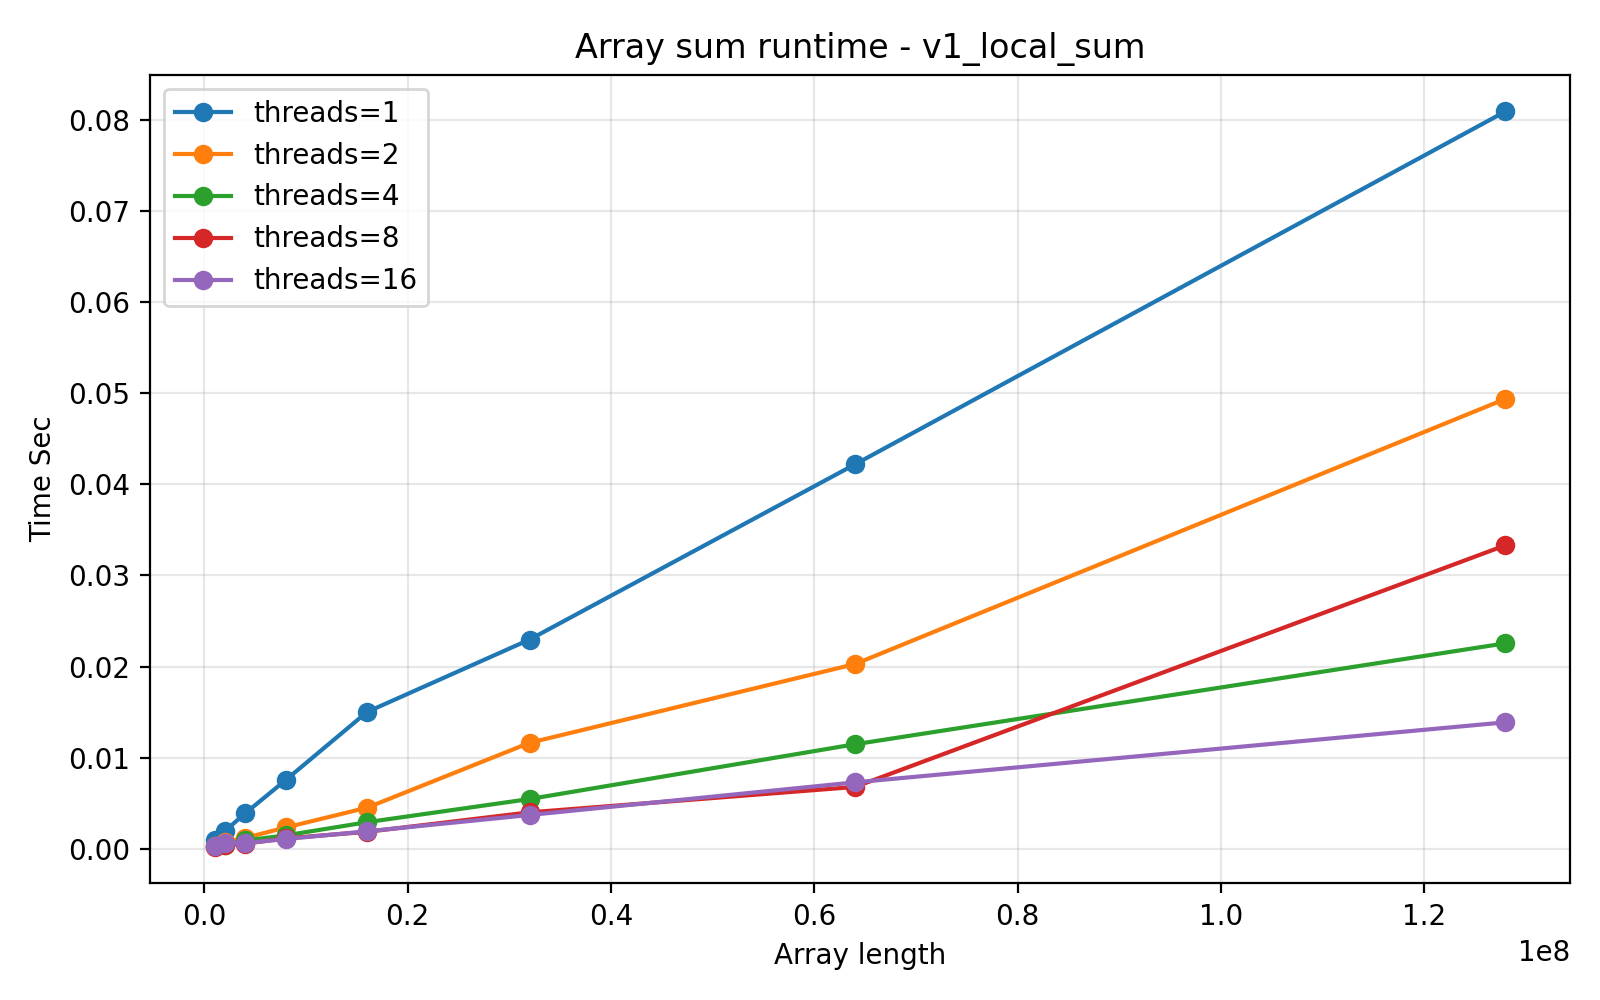
\includegraphics[width=\textwidth]{runtime_array_sum_v1_local_sum.png}
    \caption{\texttt{v1\_local\_sum} 运行时间}
  \end{subfigure}
  \hfill
  \begin{subfigure}[t]{0.48\textwidth}
    \centering
    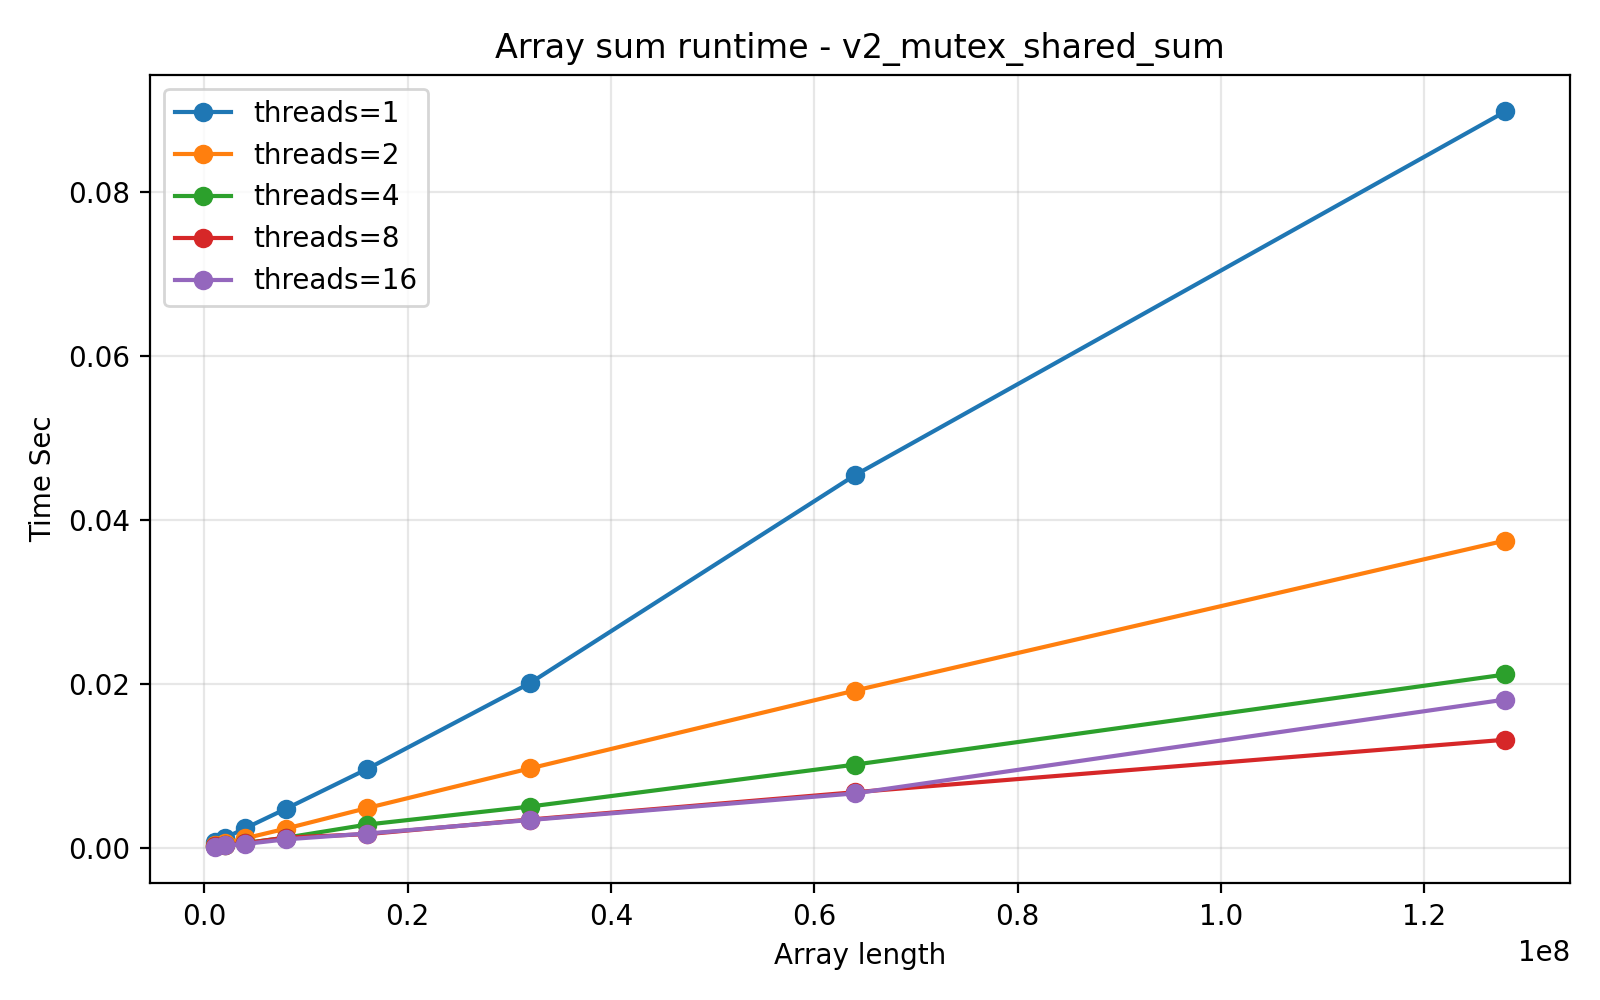
\includegraphics[width=\textwidth]{runtime_array_sum_v2_mutex_shared_sum.png}
    \caption{\texttt{v2\_mutex\_shared\_sum} 运行时间}
  \end{subfigure}
  \caption{数组求和运行时间曲线}
\end{figure}

\begin{figure}[H]
  \centering
  \begin{subfigure}[t]{0.48\textwidth}
    \centering
    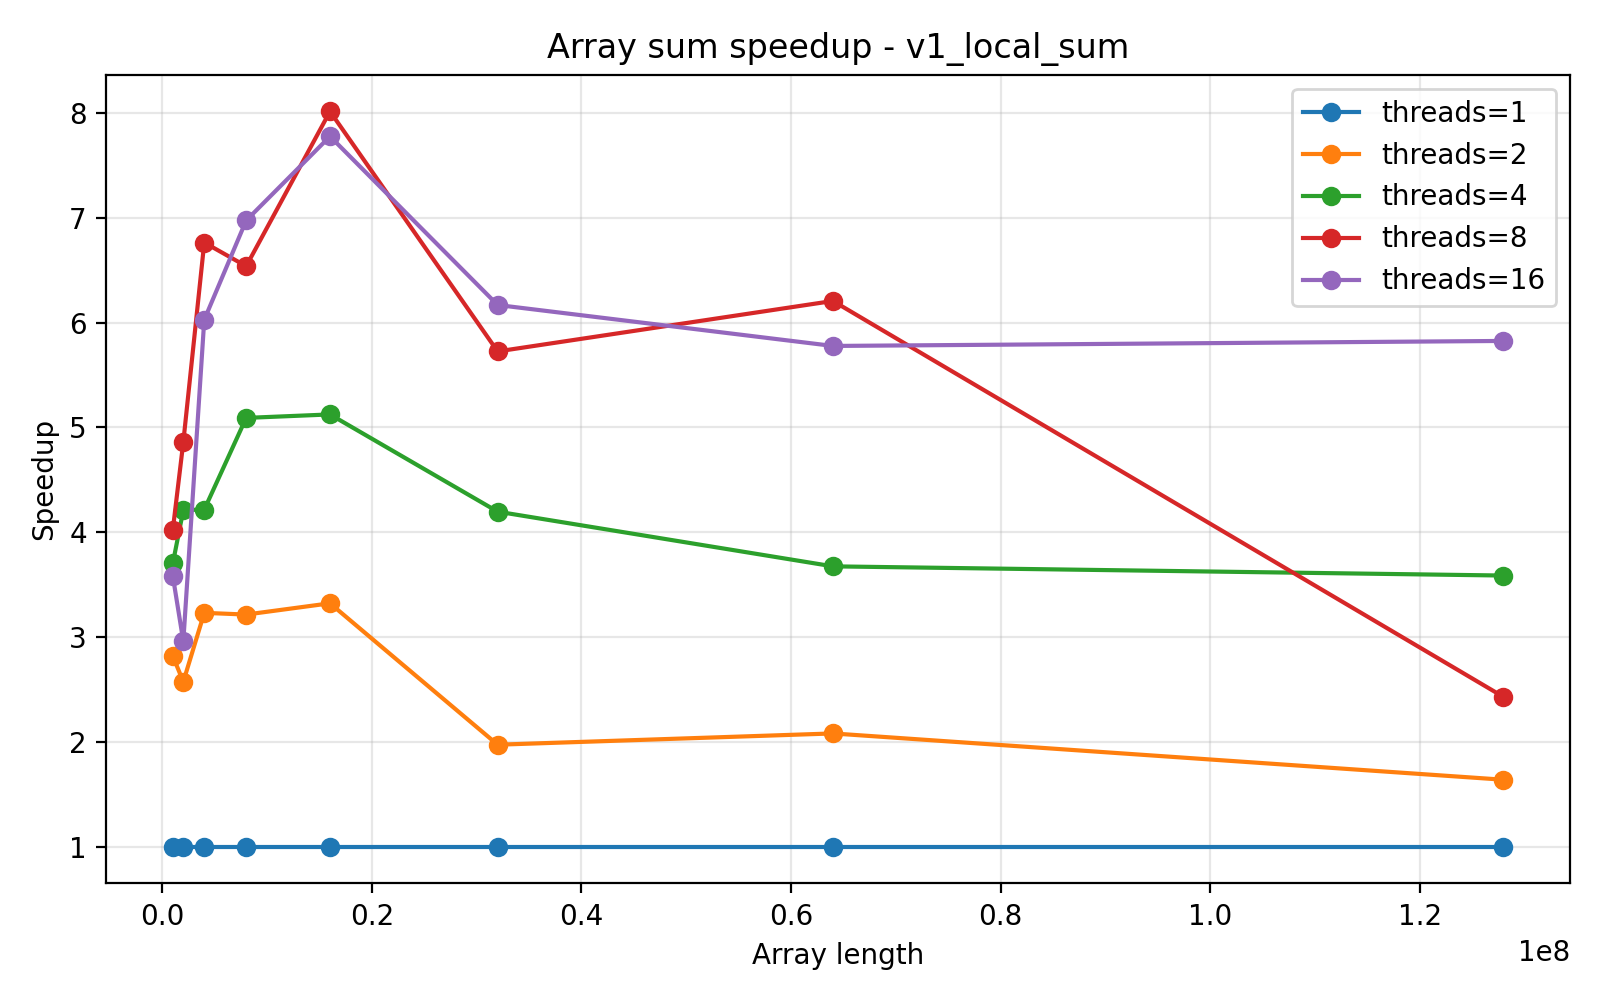
\includegraphics[width=\textwidth]{speedup_array_sum_v1_local_sum.png}
    \caption{\texttt{v1\_local\_sum} 加速比}
  \end{subfigure}
  \hfill
  \begin{subfigure}[t]{0.48\textwidth}
    \centering
    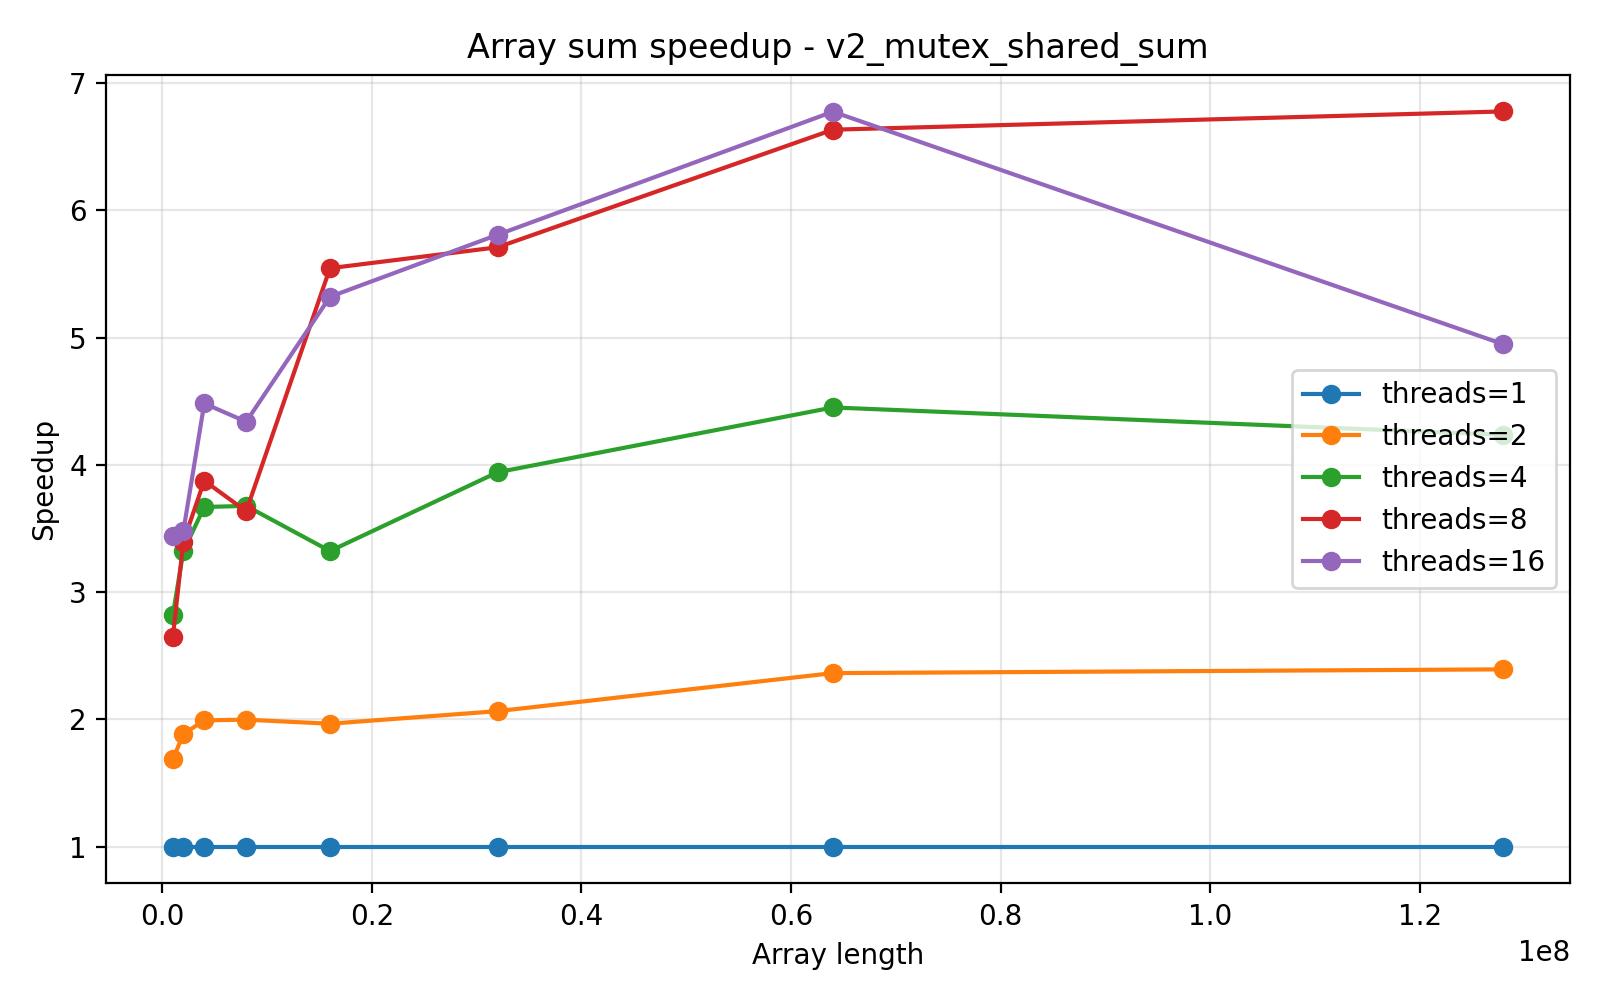
\includegraphics[width=\textwidth]{speedup_array_sum_v2_mutex_shared_sum.png}
    \caption{\texttt{v2\_mutex\_shared\_sum} 加速比}
  \end{subfigure}
  \caption{数组求和加速比曲线}
\end{figure}

数组求和的趋势比矩阵乘法更清晰。以最大长度 \(128\text{M}\) 为例，\texttt{v1\_local\_sum} 从 1 线程的 0.0809 秒下降到 16 线程的 0.0139 秒，speedup 达到 5.825；\texttt{v2\_mutex\_shared\_sum} 则从 0.0898 秒下降到 0.0182 秒，speedup 为 4.947。两者都明显受益于并行化，但 \texttt{v1} 的优势在大规模和高线程数条件下更加稳定，说明数组求和这类低计算强度、顺序访存占主导的任务，对同步开销非常敏感。

从线程扩展过程看，\texttt{v1\_local\_sum} 的增长路径更符合“先提升、后受带宽限制”的常见规律：在 \(16\text{M}\) 到 \(128\text{M}\) 范围内，其 8 线程 speedup 已能达到 8.015，16 线程 speedup 也保持在 5.825 左右。这说明这类实现主要受内存带宽与线程调度开销约束。相比之下，\texttt{v2\_mutex\_shared\_sum} 在同样规模下虽然也能随线程数增加而提速，但效率始终更低，例如在 \(128\text{M}\) 上 16 线程 efficiency 只有 0.309，而 \texttt{v1} 为 0.364。这个差距直接反映了 mutex 在归约阶段引入的串行化影响：临界区越集中，高线程数下等待与唤醒的固定成本越容易被放大。

因此，数组求和部分的核心结论非常明确：对于本质上“计算轻、访存重”的归约类任务，优先减少同步，而不是机械增加线程，往往才是更有效的优化方向。\texttt{v1\_local\_sum} 优于 \texttt{v2\_mutex\_shared\_sum}，并不是因为它做了更多计算优化，而是因为它把共享写入压缩到了最后一步，从而避免了在高频路径上引入锁竞争。

\section{性能分析}

本实验最值得注意的现象有三点。

第一，矩阵乘法并不是“线程越多越快”，更不是“线程划分越均衡越快”。从表格可以看到，\texttt{v1\_row\_block} 与 \texttt{v2\_cyclic\_rows} 都存在 speedup 随线程数增加而逐渐放缓的现象，尤其在 \(1024\) 和 \(2048\) 规模上更明显。这意味着瓶颈已经不只在算术运算本身，还转移到了缓存局部性、线程调度以及主存带宽上。对矩阵乘法而言，连续行块划分虽然在理论负载均衡上不一定更优，但其访存模式更连续，因此更容易在大规模下体现稳定优势。

第二，数组求和的核心矛盾不是“是否并行”，而是“如何归约”。\texttt{v1\_local\_sum} 基本体现了低同步开销的优势；\texttt{v2\_mutex\_shared\_sum} 虽然实现直接，但随着线程数增加，会更容易受到锁竞争影响。对这种计算量较小、访存较顺序的任务来说，减少同步往往比增加线程数本身更重要。换言之，数组求和的性能上限更多由共享更新方式决定，而不是由线程创建数量单独决定。

第三，需要正确看待实验中的“异常点”或“超线性效率”现象。无论是矩阵乘法还是数组求和，在部分小规模配置上都出现了并行效率大于 1 的结果。以数组求和为例，局部和版本在 2 线程、\(4\text{M}\) 长度下效率达到 1.615；矩阵乘法中，循环行分配版本在 \(256\) 规模下的 16 线程加速比也达到 5.830。这类结果并不意味着程序获得了“理论上超过线性”的真实长期收益，而更可能来自以下因素的叠加：其一，小规模问题本身运行时间极短，计时抖动对比值影响更大；其二，多线程运行可能更好地利用了缓存预热与系统瞬时调度机会；其三，单线程基线在极短任务上更容易受到系统后台活动干扰。因此，这些点应当被理解为实验噪声与体系结构细节共同作用下的局部现象，而不能据此得出“效率可以长期超过 100\%”的结论。

\section{总结}

本实验完成了 Pthreads 并行矩阵乘法与数组求和的代码实现、benchmark、图表、表格与中文报告闭环。整体结果说明：
\begin{enumerate}[leftmargin=2.2em]
  \item 并行化能够显著缩短大规模矩阵乘法与长数组求和的运行时间；
  \item 矩阵乘法中，连续行块静态划分通常比循环行分配更稳定，原因主要与局部性有关；
  \item 数组求和中，局部和后归并的方式通常优于 mutex 共享归约，因为同步竞争更少；
  \item 真正决定可扩展性的，不只是线程数，而是线程划分方式、同步策略与内存访问模式之间的配合程度。
\end{enumerate}

总体来看，Lab3 的结果符合并行程序设计中的常见规律：并行本身不是目的，如何组织数据与线程，才是决定性能上限的关键。

\end{document}
